\documentclass[11pt,a4paper]{article}

\usepackage[margin=1in]{geometry}
\usepackage{amsmath, amssymb, mathtools}
\usepackage{fontspec}
\IfFontExistsTF{Times New Roman}
  {\setmainfont{Times New Roman}}
  {\setmainfont{Liberation Serif}}
\IfFontExistsTF{Arial}
  {\setsansfont{Arial}}
  {\setsansfont{Liberation Sans}}
\usepackage{newunicodechar}
\newunicodechar{≈}{\ensuremath{\approx}}
\newunicodechar{≤}{\ensuremath{\leq}}
\newunicodechar{≥}{\ensuremath{\geq}}
\newunicodechar{×}{\ensuremath{\times}}
\newunicodechar{−}{\ensuremath{-}}

\usepackage{xcolor}
\definecolor{headingcolor}{HTML}{1F4E79}
\definecolor{lightgray}{HTML}{666666}

\usepackage{setspace}
\onehalfspacing
\setlength{\parindent}{0pt}
\setlength{\parskip}{0.6em}

\usepackage{titlesec}
\titleformat{\section}
{\color{headingcolor}\sffamily\Large\bfseries}
{\thesection}{1em}{}
\titleformat{\subsection}
{\sffamily\large\bfseries}
{\thesubsection}{1em}{}

\usepackage{listings}
\lstset{
    basicstyle=\ttfamily\footnotesize,
    breaklines=true,
    columns=fullflexible,
    frame=single,
    framerule=0.4pt,
    showstringspaces=false,
    xleftmargin=0.4em,
    xrightmargin=0.4em,
    aboveskip=0.5em,
    belowskip=0.5em,
}

\usepackage{booktabs}
\usepackage{graphicx}
\usepackage{caption}
\captionsetup{font=small, labelfont=bf}

\newcommand{\courseheader}{
    \begin{center}
        {\sffamily\Large\bfseries CESE5040}\\[0.3em]
        {\sffamily High-Performance and AI Architectures}\\
        {\color{lightgray}2026 Q4}
    \end{center}
}

\newcommand{\Q}[1]{\subsection*{Question #1}}
\newcommand{\Qpart}[1]{\textbf{#1.}}

\begin{document}

\courseheader
\vspace{1em}

{\color{headingcolor}\sffamily\large\bfseries Student Information}

\textbf{Name:} Daniel Tyukov\\
\textbf{Student Number:} 5714699\\
\textbf{Lab:} Lab Assignment 5

{\color{headingcolor}\sffamily\large\bfseries Notes}

\begin{itemize}\setlength\itemsep{0.1em}
    \item Model: 5-layer MLP, $16\to64\to64\to64\to10$, ReLU (10{,}058 parameters), supplied as a serialized JAX callable and a Keras file.
    \item Hardware (AWS): Intel Xeon Platinum 8259CL (4 cores / 8 threads, 2.5 GHz), NVIDIA Tesla T4 (16 GB, 70 W cap). JAX 0.10.0.
    \item TPUv2 modelled in NeuSim; FPGA is hls4ml 1.3.0 $\to$ Vitis/Vivado 2025.2 targeting an Alveo U200 (\texttt{xcu200}).
    \item CPU/GPU latencies are the minimum over 500--1000 timed calls after a warm-up dispatch (\texttt{block\_until\_ready}). GPU power is the steady-state \texttt{nvidia-smi} draw under back-to-back inference. The CPU has no usable power telemetry on a virtualised AWS host, so 100 W is assumed per the brief.
\end{itemize}

\vspace{0.5em}

\section*{\color{headingcolor}Lab Exercise 5}

% =========================================================================
\Q{5.1 - CPU and GPU single-inference latency and energy}

\begin{table}[h]
\centering
\small
\begin{tabular}{lrrr}
\toprule
Backend & Latency & Power & Energy / inference \\
\midrule
CPU & 16.6 \textmu s & 100 W (assumed) & 1.66 mJ \\
GPU & 89.5 \textmu s & 26.8 W (measured) & 2.40 mJ \\
\bottomrule
\end{tabular}
\caption{Single inference ($B=1$). GPU power is the sustained draw while looping batch-1 inferences. Energy $=$ power $\times$ latency.}
\end{table}

The CPU runs a single inference in 16.6 \textmu s against the GPU's 89.5 \textmu s, so it is 5.4$\times$ faster and, at 1.66 mJ versus 2.40 mJ, also 1.4$\times$ cheaper in energy. A batch-1 pass through a 10k-parameter MLP is a handful of tiny matrix-vector products. That offers no parallelism for the T4's 2560 CUDA cores to exploit, so the call time is dominated by kernel-launch and host-device dispatch overhead while the GPU sits near its 27 W idle floor. The CPU keeps everything in cache and avoids that overhead entirely. For latency-critical single inference of a small model, the CPU is the better device.

% =========================================================================
\Q{5.2 - CPU and GPU throughput}

Batched inference only needs the input widened from $(1,16)$ to $(B,16)$; the same jitted function then processes $B$ samples per call. Sweeping $B$ gives the throughput in Figure~\ref{fig:thr}.

\begin{table}[h]
\centering
\small
\begin{tabular}{lrrrr}
\toprule
Backend & Max throughput & at batch & Power & Throughput / W \\
\midrule
CPU & 12.9 M inf/s & 40{,}960 & 100 W (assumed) & 0.13 M inf/s/W \\
GPU & 52.9 M inf/s & 262{,}144 & 70 W (measured) & 0.76 M inf/s/W \\
\bottomrule
\end{tabular}
\caption{Peak throughput. GPU energy at peak is 1.32 \textmu J/inference; the GPU draws its full 70 W cap under load.}
\end{table}

\begin{figure}[h]
\centering
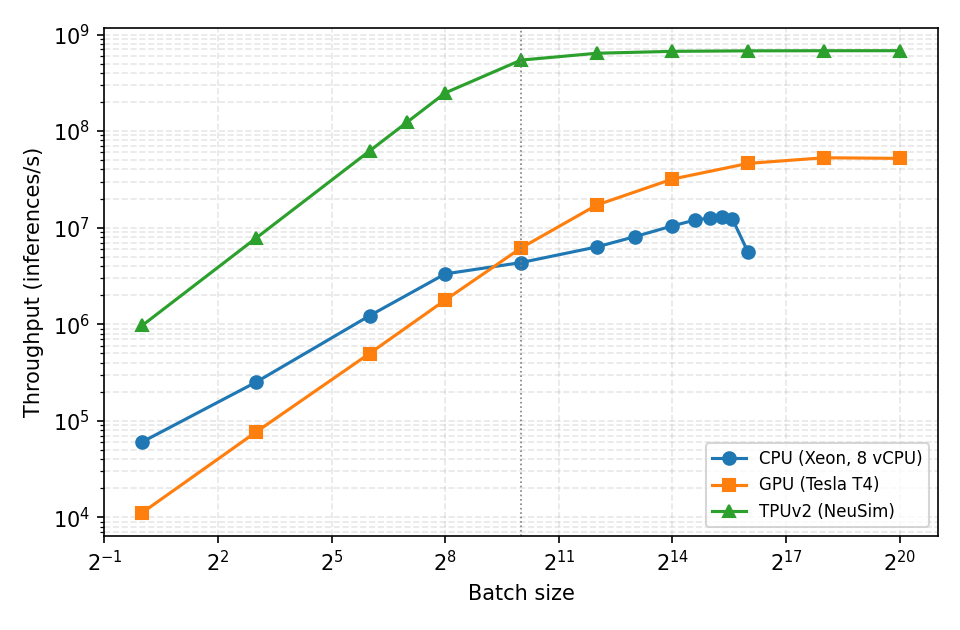
\includegraphics[width=0.72\linewidth]{../figures/throughput_sweep.png}
\caption{Throughput versus batch size (log-log), including the TPU from 5.4. The CPU leads below $B\approx1024$ (dotted line); the GPU then overtakes it and peaks 4.1$\times$ higher. CPU throughput collapses past $B=40{,}960$ once the working set spills out of cache.}
\label{fig:thr}
\end{figure}

The GPU reaches 52.9 M inf/s, 4.1$\times$ the CPU's 12.9 M inf/s, and at its peak is 5.8$\times$ more energy-efficient (1.32 \textmu J versus 7.8 \textmu J per inference). But the two crossover only at $B\approx1024$: below that the CPU wins, because the GPU cannot fill its cores. The takeaway across 5.1 and 5.2 is that the right device depends on the access pattern, not the peak FLOPS. One-at-a-time inference of a small model belongs on the CPU; only large-batch, high-volume serving justifies the GPU, and even then this model is so small that batches of $\sim10^5$ are needed before the hardware saturates.

% =========================================================================
\Q{5.3 - Roles of the systolic array and vector unit}

The \textbf{systolic array (MXU)} is a 2-D grid of multiply-accumulate cells (128$\times$128 in TPUv2) built for dense matrix multiplication. Operands are pumped in from two edges and partial sums ripple through the array, so each value loaded into the grid is reused across a whole row or column of MACs. This data reuse is what gives the TPU its enormous GEMM throughput at low energy per operation, and it is where the matmul-heavy layers (the Linear/convolution work) execute.

The \textbf{vector unit (VPU)} is a SIMD ALU array for the elementwise and reduction work that does not map onto a matrix multiply: activations (ReLU here), bias adds, normalisation, softmax, and pooling. It is far smaller than the MXU in raw throughput but flexible. In short, the MXU does the heavy linear algebra and the VPU does the per-element math that surrounds it.

% =========================================================================
\Q{5.4 - TPUv2 in NeuSim}

\Qpart{1} For a single inference the five layers run as five memory-bound MXU einsums of 206 ns each, summarised in Table~\ref{tab:tpu1}.

\begin{table}[h]
\centering
\small
\begin{tabular}{lrrr}
\toprule
 & Execution time & Power & Energy \\
\midrule
TPUv2, $B=1$ & 1030 ns & 91.0 W & 93.7 \textmu J \\
\bottomrule
\end{tabular}
\caption{Single inference on TPUv2. Power is the energy-weighted average reported by NeuSim; static (leakage) power dominates because the matmuls are tiny.}
\label{tab:tpu1}
\end{table}

\Qpart{2} Sweeping the batch size, latency stays flat at 1030 ns up to $B=256$ (the run is memory-bound, so more samples cost no extra time) and throughput rises linearly. From $B\approx1024$ the run turns compute-bound and latency grows with $B$, so throughput saturates at roughly \textbf{680 M inf/s} (Figure~\ref{fig:thr}, and the latency knee in Figure~\ref{fig:roof}).

\Qpart{3} Table~\ref{tab:cmp} collects all three backends.

\begin{table}[h]
\centering
\small
\begin{tabular}{lrrr}
\toprule
 & CPU & GPU & TPUv2 \\
\midrule
Single-inference latency & 16.6 \textmu s & 89.5 \textmu s & 1.03 \textmu s \\
Max throughput (inf/s) & 12.9 M & 52.9 M & 680 M \\
Single-inference energy & 1.66 mJ & 2.40 mJ & 93.7 \textmu J \\
Power at peak throughput & 100 W$^\ast$ & 70 W & 105.5 W \\
Energy / inference at peak & 7.8 \textmu J & 1.32 \textmu J & 0.155 \textmu J \\
Throughput / W at peak & 0.13 M & 0.76 M & 6.44 M \\
\bottomrule
\end{tabular}
\caption{Cross-backend comparison. $^\ast$CPU power assumed. TPU figures are NeuSim's on-chip device model and exclude host overhead, which is why its single-inference latency undercuts the measured CPU/GPU numbers.}
\label{tab:cmp}
\end{table}

The TPU wins on every axis for this workload: 12.9$\times$ the GPU's throughput, 26$\times$ lower single-inference energy, and 8.5$\times$ the GPU's throughput-per-watt at peak. Its single-inference latency (1.03 \textmu s) is the lowest of the three, though that is the modelled device time only; the CPU and GPU numbers include real host dispatch, so the gap to a deployed TPU would be smaller. The pattern from 5.2 repeats: against a purpose-built matrix engine the general-purpose GPU is badly underused by such a small model.

% =========================================================================
\Q{5.5 - Reading the TPU results}

\Qpart{1} Every layer of this MLP is a matrix multiply, so all five operators run on the \textbf{MXU}. The \textbf{VPU} carries the small elementwise work attached to each layer: the ReLU activations and bias adds (3--5 ns per op in the trace). On a larger network the VPU would also own softmax, layer-norm and pooling.

\Qpart{2} At $B=1$ each layer multiplies a $1\times64$ activation by a $64\times64$ weight. The arithmetic is trivial (compute time 114 ns) but the weights must still be streamed from memory (206 ns), and they are reused only once, so the run is \textbf{memory-bound}. Batching reuses the same weight matrix across all $B$ rows: the weight-load cost is fixed while compute scales with $B$, so arithmetic intensity rises and by $B\approx1024$ compute time overtakes memory time and the run becomes \textbf{compute-bound} (Figure~\ref{fig:roof}). This is the standard low-vs-high arithmetic-intensity transition on the roofline.

\begin{figure}[h]
\centering
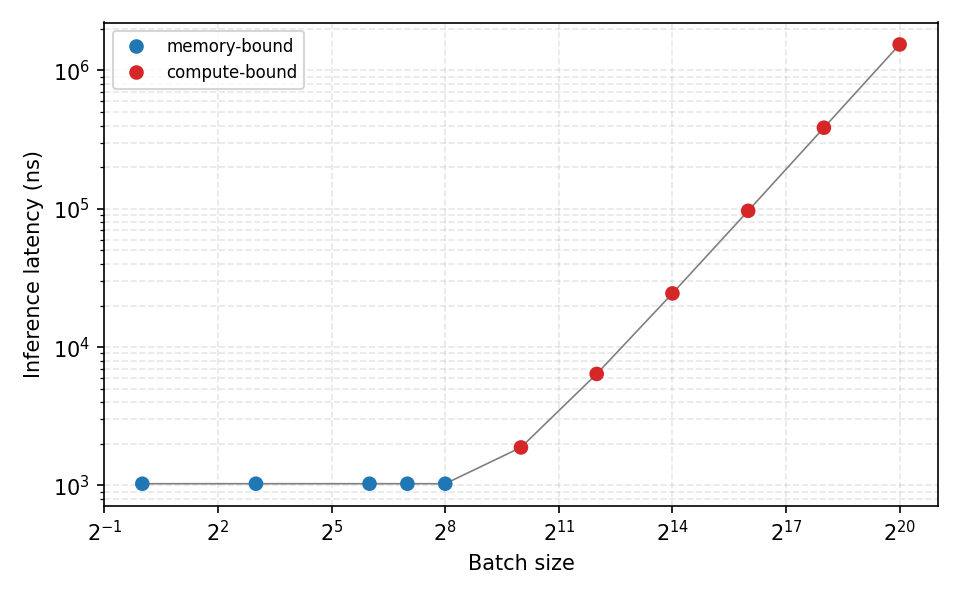
\includegraphics[width=0.66\linewidth]{../figures/tpu_roofline.png}
\caption{TPUv2 per-inference latency versus batch size. Latency is flat (memory-bound) while the matmul underfills the array, then grows once the run becomes compute-bound near $B=1024$.}
\label{fig:roof}
\end{figure}

\Qpart{3} With \texttt{use\_vu\_for\_small\_matmul = false} the matmuls run on the MXU; setting it \texttt{true} reroutes them to the VPU. Latency is identical at 1030 ns either way, because the run is memory-bound and moving the matmul off the MXU does not touch the bottleneck. Energy, though, drops from 93.7 \textmu J to 91.9 \textmu J (power 91.0 W $\to$ 89.2 W). A $1\times64$ by $64\times64$ matmul fills only one of the 128 systolic rows, so spinning up the full array wastes dynamic energy; the VPU does the same tiny multiply more cheaply. NeuSim shows the MXU time collapsing from 114 ns to 0 while the VPU absorbs the work.

% =========================================================================
\Q{5.6 - hls4ml architecture and reuse factor}

hls4ml emits a \textbf{fully-unrolled, layer-pipelined dataflow} design: every layer (dense, activation) becomes its own hardware block, the blocks are wired front-to-back as a feed-forward pipeline, and all weights live in on-chip BRAM/LUTs so there is no external memory in the inference loop. With pipelining, several inferences are in flight at once.

The \textbf{reuse factor (RF)} is the number of multiplications mapped onto a single physical multiplier, i.e.\ how many times each multiplier is time-shared within a layer: $n_{\text{mult}} = (n_{\text{in}}\cdot n_{\text{out}})/\text{RF}$. RF\,=\,1 is fully parallel, one multiplier per multiplication, giving the lowest latency and an initiation interval of 1 at maximum resource cost. Increasing RF serialises the multiplications onto fewer multipliers, cutting resource use by roughly RF$\times$ while raising the latency and initiation interval by the same factor. It is the core latency-versus-area knob of the framework.

% =========================================================================
\Q{5.7 - FPGA synthesis at default settings}

\Qpart{1} Default design: \texttt{ap\_fixed<8,4>}, reuse factor 1, 5 ns clock (200 MHz). The synthesis report gives:

\begin{table}[h]
\centering
\small
\begin{tabular}{lrr}
\toprule
Metric & Value & \\
\midrule
Latency & 10 cycles & 50.0 ns \\
Initiation interval & 1 cycle & pipelined \\
\midrule
DSP & 0 & 0\% \\
BRAM\_18K & 0 & 0\% \\
Flip-flops & 16{,}215 & 2\% (SLR) \\
LUTs & 148{,}931 & 37\% (SLR) \\
\bottomrule
\end{tabular}
\caption{Default HLS synthesis result (Alveo U200). The estimated clock (3.35 ns) meets the 5 ns target.}
\label{tab:fpga_default}
\end{table}

The design uses \textbf{zero DSPs}: at 8-bit fixed point the multipliers are small enough that Vitis packs them into LUT fabric, so the LUT count (37\% of one SLR) is the binding resource while the 6840 DSP blocks go unused.

\Qpart{2} The initiation interval is 1 cycle, so a new inference can start every clock. The end-to-end latency of $N$ back-to-back inferences is
\[
T(N) = \big(L + (N-1)\cdot\text{II}\big)\cdot T_{\text{clk}} = (10 + (N-1))\cdot 5\ \text{ns} = (N+9)\cdot 5\ \text{ns},
\]
e.g.\ 5045 ns for $N=1000$. Throughput is $1/(\text{II}\cdot T_{\text{clk}}) = 1/5\ \text{ns} = \mathbf{2.0\times10^{8}}$ \textbf{inf/s} (200 M inf/s), set by the clock and the unit initiation interval rather than the 50 ns pipeline depth.

% =========================================================================
\Q{5.8 - Frequency, precision, and reuse factor}

\Qpart{1} \textit{Clock at 10 ns (100 MHz), default precision.} The latency drops to \textbf{30.0 ns} (3 cycles), down from 50.0 ns (10 cycles) at 200 MHz, and the flip-flop count falls from 16{,}215 to 1{,}670. This looks backwards until you remember that absolute latency is cycles $\times$ period. A 10 ns clock gives the scheduler twice the time budget per cycle (the estimated path is 6.75 ns), so it packs the same logic into 3 pipeline stages instead of 10 and needs far fewer pipeline registers. $3\times10 = 30$ ns beats $10\times5 = 50$ ns: halving the frequency actually lowers end-to-end latency here. The cost is throughput, which is set by the unit initiation interval at the clock rate and so halves from 200 M to 100 M inf/s.

\Qpart{2} \textit{Precision Q2.2 (\texttt{ap\_fixed<4,2>}) at 200 MHz.}

\begin{table}[h]
\centering
\small
\begin{tabular}{lrrr}
\toprule
Design & Latency & LUTs & Flip-flops \\
\midrule
Default \texttt{ap\_fixed<8,4>} & 50.0 ns (10 cyc) & 148{,}931 & 16{,}215 \\
Q2.2 \texttt{ap\_fixed<4,2>} & 35.0 ns (7 cyc) & 36{,}076 & 3{,}630 \\
\bottomrule
\end{tabular}
\caption{Halving the word length cuts LUTs 4.1$\times$ and FFs 4.5$\times$, and trims latency to 7 cycles. DSP and BRAM stay at zero.}
\end{table}

Narrower operands mean smaller multipliers and adders and shorter carry chains, so each operation needs less logic (the 4$\times$ LUT drop) and fits in fewer pipeline stages (10$\to$7). The downside is numerical: Q2.2 has 2 integer and 2 fractional bits, i.e.\ a range of only $[-2, 1.75]$ at a resolution of 0.25. Weights or activations outside that range saturate and everything else is coarsely rounded, so beyond a point aggressive quantisation trades accuracy for the area and latency it saves.

\Qpart{3} \textit{Reuse factor 4 at default precision, 200 MHz.} Raising RF from 1 to 4 should time-share each multiplier across 4 multiplications: I expected roughly 4$\times$ fewer multipliers, an initiation interval near 4, and a longer latency. The synthesis report only partly bears this out. The initiation interval rises to \textbf{2} (not 4), latency stays at 50.0 ns (10 cycles), and the resource use is essentially unchanged: 149{,}005 LUTs and 16{,}213 FFs against the default's 148{,}931 and 16{,}215.

The reason is that the reuse factor saves area by sharing scarce \emph{DSP} multipliers, but this design has DSP\,=\,0: the 8-bit multipliers are already small LUT logic that the tool does not fold further, so RF buys no LUT reduction. What it does change is scheduling: each dense layer now accepts a new input every 2 cycles, so throughput halves to $1/(2\cdot5\,\text{ns}) = \mathbf{1.0\times10^{8}}$ \textbf{inf/s} (100 M inf/s) and the back-to-back latency becomes $T(N) = (10 + (N-1)\cdot2)\cdot5 = (10N+40)$ ns. The takeaway is that the reuse factor only pays off when a design is multiplier-bound; for this LUT-bound 8-bit design it trades throughput for nothing.

% =========================================================================
\Q{5.9 - Vivado power}

Running \texttt{report\_power} after a Vivado synthesis of the default design (default precision, reuse 1) at both clocks gives the figures in Table~\ref{tab:power} (vectorless estimate, ``Low'' confidence, as the brief notes).

\begin{table}[h]
\centering
\small
\begin{tabular}{lrrrrrr}
\toprule
Clock & Latency & Throughput & Total power & (dyn / static) & Energy / inf & Throughput / W \\
\midrule
200 MHz & 50 ns & 200 M inf/s & 6.40 W & 3.88 / 2.52 W & 0.32 \textmu J & 31.3 M inf/s/W \\
100 MHz & 30 ns & 100 M inf/s & 6.42 W & 3.90 / 2.52 W & 0.19 \textmu J & 15.6 M inf/s/W \\
\bottomrule
\end{tabular}
\caption{Vivado power for the default design. Energy/inference $=$ power $\times$ latency; throughput/W $=$ throughput $\div$ power.}
\label{tab:power}
\end{table}

The two designs draw almost the same total power (6.40 vs 6.42 W), which is the surprise: halving the clock barely moved it. Two things explain this. Static power (2.52 W, $\approx40\%$ of the total) is frequency-independent. And the dynamic estimate is vectorless, so Vivado applies a default switching activity rather than a real workload trace; the 100 MHz design also trades pipeline registers for deeper combinational logic (3 stages vs 10), so more logic toggles per cycle and the lower clock rate is largely cancelled.

Given near-equal power, the two metrics point in opposite directions. For a \textbf{single inference}, 100 MHz is more energy-efficient (0.19 vs 0.32 \textmu J) purely because its latency is lower (30 vs 50 ns). For \textbf{back-to-back throughput}, 200 MHz wins decisively at 31.3 vs 15.6 M inf/s/W, because it retires twice as many inferences per second for the same power. When the workload is a stream, run the clock as fast as it will close; when it is one-shot and latency-bound, the shorter pipeline wins. Either way the FPGA's throughput-per-watt is far above the GPU (0.76 M/W) and TPU (6.44 M/W) for this fixed, quantised datapath.

% =========================================================================
\Q{5.10 - Choosing a platform}

No single device wins everywhere; the choice follows the workload.

\begin{itemize}\setlength\itemsep{0.15em}
    \item \textbf{Training} favours GPUs and TPUs: it is throughput-bound, runs at large batch, needs high-precision floating point and frequent model changes. GPUs are the default for their generality and software maturity; TPUs pull ahead at large scale on matmul-dominated models (as the 8.5$\times$ throughput-per-watt edge in Table~\ref{tab:cmp} shows). FPGAs and fixed accelerators are ill-suited, since re-synthesising for every architecture change is impractical.
    \item \textbf{Inference} depends on volume and latency. One-off or low-rate inference of a small model belongs on a \textbf{CPU}: lowest latency, lowest energy, no batching needed (5.1). High-volume datacentre serving belongs on a \textbf{GPU or TPU}, where batching amortises the hardware and the TPU's efficiency dominates for stable, matmul-heavy models.
    \item \textbf{Edge and real-time} inference, where latency is hard-bounded and a power budget is tight, favours the \textbf{FPGA}: a fixed, deterministic 50 ns per inference at 200 M inf/s on a known-small model (5.7), with quantisation (5.8) trading accuracy for area and energy. The cost is flexibility: the design is re-synthesised per model and per precision.
    \item \textbf{Model size and generality} set the outer limits. Large, irregular or fast-changing models want the programmability of GPUs/TPUs; small, fixed, high-rate kernels reward the FPGA's custom datapath; latency-sensitive single-shot work stays on the CPU.
\end{itemize}

In short: CPU for low-rate small-model inference, GPU for general training and flexible serving, TPU for large-scale matmul throughput and efficiency, FPGA for fixed low-latency energy-constrained inference at the edge.

% =========================================================================

\vspace{1em}

{\color{headingcolor}\sffamily\large\bfseries LLM Usage Disclosure}

\vspace{0.3em}

I used Claude Code on this lab for:
\begin{itemize}
    \item Cross-checking the hls4ml reuse-factor and TPU MXU/VPU descriptions against the documentation.
    \item Editing the report for concision.
\end{itemize}

\end{document}
